\apendice{Especificación Técnica}
\label{apendice:C}

\section{Introducción}
En este anexo se presenta la especificación técnica del sistema. Se detallan las decisiones tomadas respecto al almacenamiento de datos, la arquitectura de software utilizada y el diseño de la interfaz gráfica, explicando cómo se han transformado los requisitos definidos anteriormente en una solución real y funcional.

\section{Diseño de Datos}
La persistencia del sistema se sustenta sobre una base de datos relacional implementada en PostgreSQL\cite{postgresql_docs}. Se ha optado por este motor debido a su estricto cumplimiento del estándar SQL y su capacidad para gestionar tipos de datos complejos y restricciones de integridad avanzadas, fundamentales para un entorno clínico donde la consistencia de los datos es crítica.

El diseño sigue una arquitectura de esquema normalizado para evitar redundancias y anomalías de actualización. A continuación, se detallan los aspectos técnicos de la implementación.

\subsection{Diagrama Entidad-Relación}

\begin{figure}[hbt]
    \centering
    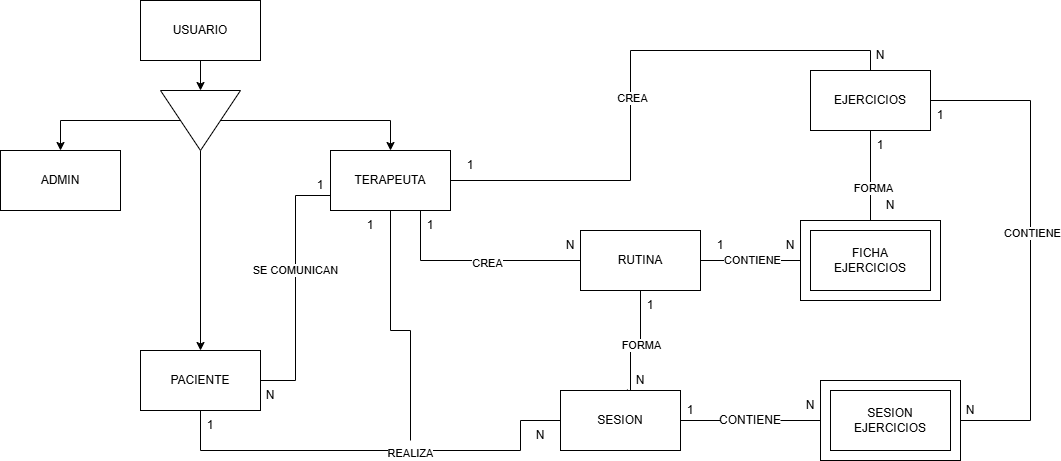
\includegraphics[width=1\textwidth]{img/Diagrama_EntidadRelacion/EntidadRelacion.png}
    \caption{Diagrama Entidad-Relación de la base de datos}
    \label{fig:diagrama_er}
\end{figure}

\subsection{Definición de entidades y atributos}
La estructura física se compone de 7 tablas principales(fig.~\ref{fig:diagrama_er}). A continuación se detallan las decisiones de diseño más relevantes para cada entidad:

\begin{enumerate}
    \item \textbf{Tabla usuario} \\
    Centraliza la información de todos los actores del sistema. Se ha optado por una estrategia de ``Tabla Única'' (Single Table Inheritance) para simplificar la autenticación.
    \begin{description}
        \item[Clave Primaria:] \texttt{id\_usuario} (SERIAL). Se utiliza una clave subrogada autoincremental para optimizar las uniones (JOINs) frente al uso del DNI.
        \item[Claves Candidatas:] Se establecen restricciones UNIQUE sobre \texttt{dni} y \texttt{correo\_electronico} para garantizar que no existan duplicidades de identidad física.
        \item[Seguridad:] El campo \texttt{contrasena} se define como VARCHAR(100) para alojar el hash generado por Bcrypt, nunca el texto plano.
    \end{description}

    \item \textbf{Tablas rutina y ejercicio} \\
    Separan la definición del ejercicio de su agrupación lógica.
    \begin{description}
        \item[Separación de Conceptos:] La tabla \texttt{ejercicio} actúa como un catálogo maestro inmutable, mientras que \texttt{rutina} actúa como contenedor.
        \item[Multimedia:] El campo \texttt{video\_prueba} almacena la ruta del vídeo. Esta decisión de diseño se tomó para mantener la base de datos ligera y delegar la gestión de archivos pesados al sistema de ficheros.
    \end{description}

    \item \textbf{Tabla ficha\_ejercicios} \\
    Resuelve la relación de cardinalidad N:M entre Rutinas y Ejercicios.

    \item \textbf{Tabla sesion} \\
    Registra la actividad.
    \begin{description}
        \item[Trazabilidad:] Vincula al paciente (\texttt{id\_paciente}), al terapeuta responsable (\texttt{id\_terapeuta}) y a la rutina utilizada (\texttt{id\_rutina}).
        \item[Estado:] Utiliza un campo de tipo enumerado para controlar el ciclo de vida de la sesión, impidiendo estados inválidos.
    \end{description}

    \item \textbf{Tabla sesión\_ejercicios} \\
    Registra los videos de los diferentes ejercicios que forman la sesión.
    \begin{description}
        \item[Persistencia Multimedia:] Almacena la ruta de los vídeos (\texttt{video\_url}) generados por el paciente.
        \item[Integridad de Datos:] Resuelve la relación técnica entre la sesión y los ejercicios realizados. Es fundamental para vincular inequívocamente cada vídeo grabado con el tipo de ejercicio específico (\texttt{id\_ejercicio}) al que corresponde.
    \end{description}
\end{enumerate}

\subsection{Tipos de datos personalizados}
Para garantizar la integridad del dominio y evitar errores de inserción, se han definido tipos enumerados específicos en PostgreSQL en lugar de utilizar cadenas de texto libre.

\begin{description}
    \item[\texttt{rol\_tipo}:] Restringe los valores a ('admin', 'terapeuta', 'paciente'). Esto es vital para la lógica de autorización de la API.
    
    \item[\texttt{zona\_tipo}:] Clasifica los ejercicios en ('Torso', 'Cabeza', 'Extremidades\_Superiores', 'Extremidades\_Inferiores'), facilitando el filtrado en la interfaz de usuario.
    
    \item[\texttt{estado\_sesion}:] Define la máquina de estados de la terapia:
    \begin{itemize}
        \item 'pendiente': Asignada pero no realizada.
        \item 'realizada': El paciente ha subido el vídeo.
        \item 'corregida': El terapeuta ha evaluado la sesión.
    \end{itemize}
\end{description}

\subsection{Integridad Referencial y Reglas de Negocio}
El diseño implementa restricciones fuertes a nivel de base de datos para asegurar la consistencia lógica del sistema médico:

\begin{itemize}
    \item En la tabla \texttt{usuario}, el campo \texttt{id\_terapeuta\_asignado} es una clave foránea que referencia a la misma tabla (usuario). Esto modela la relación jerárquica ``Paciente pertenece a Terapeuta'', permitiendo que un terapeuta supervise a múltiples pacientes, pero un paciente solo tenga un responsable principal.
    
    \item Se ha configurado la regla ON DELETE CASCADE en la relación \texttt{fk\_ficha\_rutina}.
    \begin{itemize}
        \item Si un terapeuta elimina una rutina, el sistema borra automáticamente todas las líneas de detalle asociadas en \texttt{ficha\_ejercicios}.
        \item Sin embargo, no se aplica cascada en los ejercicios. Si se borra una rutina, los ejercicios base permanecen en la biblioteca para no afectar a otras rutinas que los utilicen.
    \end{itemize}
    
    \item La tabla \texttt{sesion} mantiene claves foráneas independientes hacia el paciente y el terapeuta. Esto asegura que, incluso si cambia la asignación de terapeuta en el futuro, el historial clínico pasado mantenga la referencia al profesional que supervisó esa sesión específica en ese momento.
\end{itemize}
\section{Diseño procedimental}
Mientras que el diseño de datos (Apartado \ref{apendice:C}.2) define la estructura estática de la información, el diseño procedimental detalla la dinámica del sistema: cómo interactúan los componentes software para satisfacer los requisitos funcionales. Para modelar el comportamiento del sistema y el intercambio de mensajes entre la aplicación móvil, la API REST y la Base de Datos, se han elaborado Diagramas de Secuencia UML\cite{uml_spec}.

A continuación, se describen los flujos de ejecución críticos, organizados por módulos funcionales.

\subsection{Módulo de seguridad y gestión de usuarios}
Este bloque abarca los procesos de autenticación y la administración de identidades, garantizando que solo los actores autorizados accedan a los recursos.

\begin{enumerate}
    \item \textbf{El acceso al sistema} está protegido mediante el estándar JSON Web Token (JWT)\cite{rfc7519_jwt}. Como se muestra en la Figura \ref{fig:ds_login}, el cliente no mantiene una sesión abierta en el servidor, sino que intercambia credenciales por un token firmado que validará las peticiones subsiguientes.
    
    \begin{figure}[hbt]
        \centering
        
\includegraphics[width=1\textwidth]{Diagramas_Secuenciales/DS-iniciarsesion.png}
        \caption{Diagrama de Secuencia: Inicio de Sesión}
        \label{fig:ds_login}
    \end{figure}

    \item \textbf{Alta de usuarios.} La creación de nuevos perfiles es una operación privilegiada. La Figura \ref{fig:ds_crear_usuario} ilustra cómo la API verifica el token del solicitante para asegurar que posee el rol de 'Administrador' antes de procesar el alta, gestionando además la lógica de no duplicidad de DNI/Correo y el cifrado de la contraseña.
    
    \begin{figure}[hbt]
        \centering
        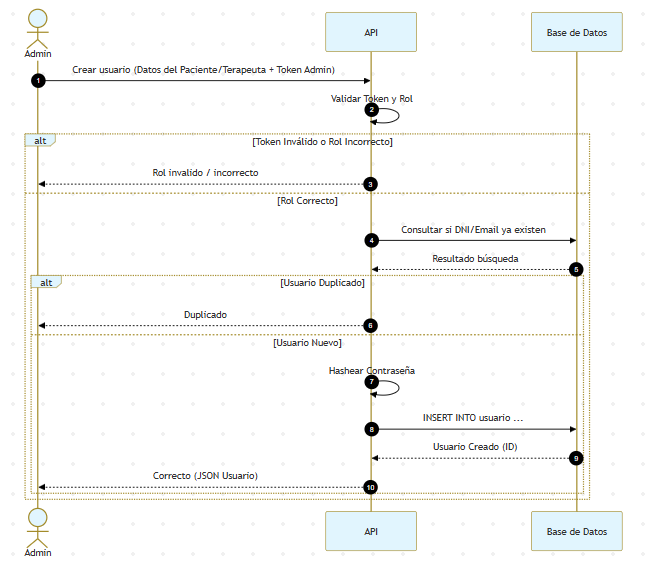
\includegraphics[width=1\textwidth]{img/Diagramas_Secuenciales/DS-crearusuario.png}
        \caption{Diagrama de Secuencia: Alta de Usuario}
        \label{fig:ds_crear_usuario}
    \end{figure}

    \item \textbf{Asignación Paciente-Terapeuta.} Para que el sistema funcione, debe existir una relación lógica entre profesional y paciente. La Figura \ref{fig:ds_asignar_paciente} detalla la transacción que actualiza la clave foránea en el perfil del usuario, estableciendo la jerarquía de supervisión.
    
    \begin{figure}[hbt]
        \centering
        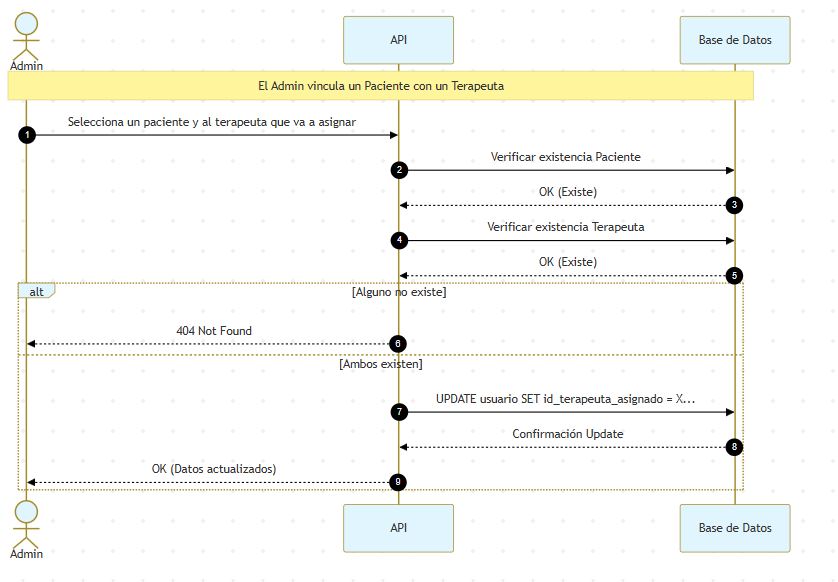
\includegraphics[width=1\textwidth]{img/Diagramas_Secuenciales/DS-asignarpaciente.png}
        \caption{Diagrama de Secuencia: Asignación de Paciente}
        \label{fig:ds_asignar_paciente}
    \end{figure}

    \item \textbf{Creación de rutinas y ejercicios.} la definición de una rutina es un proceso transaccional de dos fases, tal como se observa en la Figura \ref{fig:ds_crear_rutina}. Primero se crea la cabecera de la rutina (nombre, descripción) y, una vez obtenido su identificador, el sistema itera para insertar las fichas de ejercicios asociadas, garantizando la integridad de la composición.
    
    \begin{figure}[hbt]
        \centering
        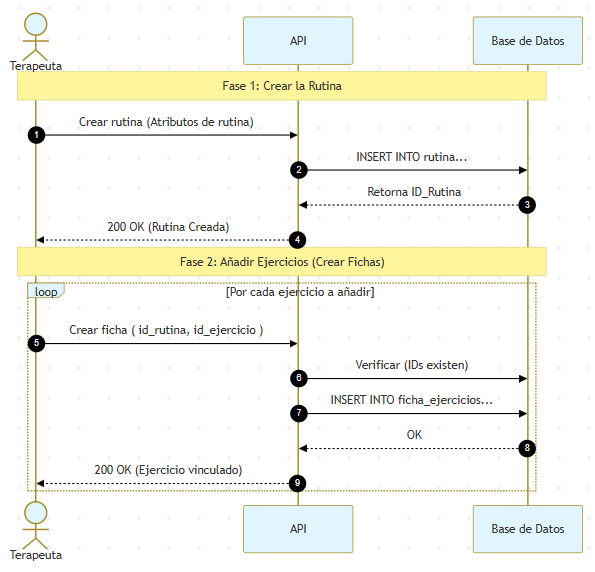
\includegraphics[width=1\textwidth]{img/Diagramas_Secuenciales/DS-crearrutina.png}
        \caption{Diagrama de Secuencia: Creación de Rutina}
        \label{fig:ds_crear_rutina}
    \end{figure}

    \item \textbf{Ciclo sesión: programación, ejecución y evaluación.} La Figura \ref{fig:ds_ciclo_completo} representa la trazabilidad completa del servicio:
    \begin{itemize}
        \item \textbf{Programación:} el terapeuta genera la cita en la base de datos (INSERT).
        \item \textbf{Ejecución:} el paciente consulta sus tareas pendientes y, tras realizar el ejercicio, el sistema gestiona la subida del vídeo (UPDATE con la ruta del archivo).
        \item \textbf{Cierre:} el terapeuta visualiza la evidencia y cierra el ciclo asignando una puntuación y validación.
    \end{itemize}
    
    \begin{figure}[hbt]
        \centering
        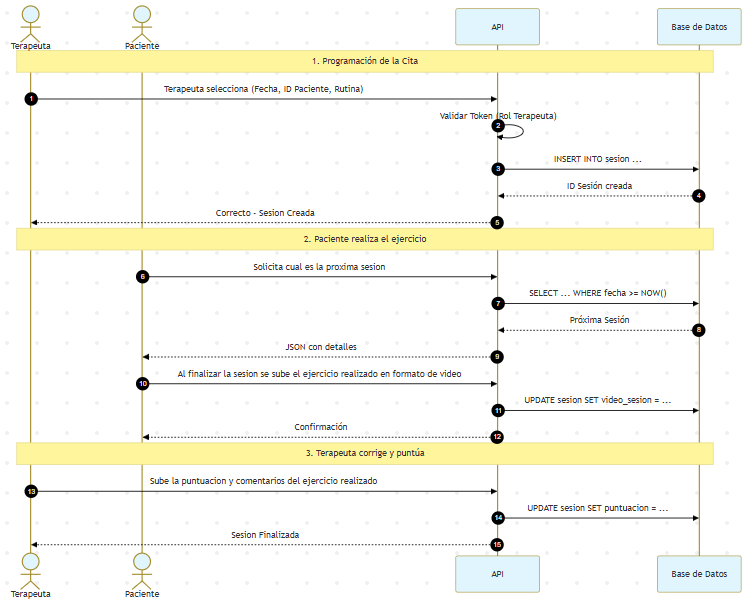
\includegraphics[width=1\textwidth]{img/Diagramas_Secuenciales/DS-cicloenterosesion.png}
        \caption{Diagrama de Secuencia: Ciclo completo de sesión}
        \label{fig:ds_ciclo_completo}
    \end{figure}

    \item \textbf{Consulta de progreso.} A diferencia de una lectura simple, la Figura \ref{fig:ds_consultar_progreso} muestra cómo el servidor procesa los datos en bruto. La API recupera el histórico de sesiones del paciente y realiza cálculos de agregación (nota media, total de sesiones, máximos) antes de devolver la respuesta al cliente, optimizando así el consumo de datos y batería en el dispositivo móvil.
    
    \begin{figure}[hbt]
        \centering
        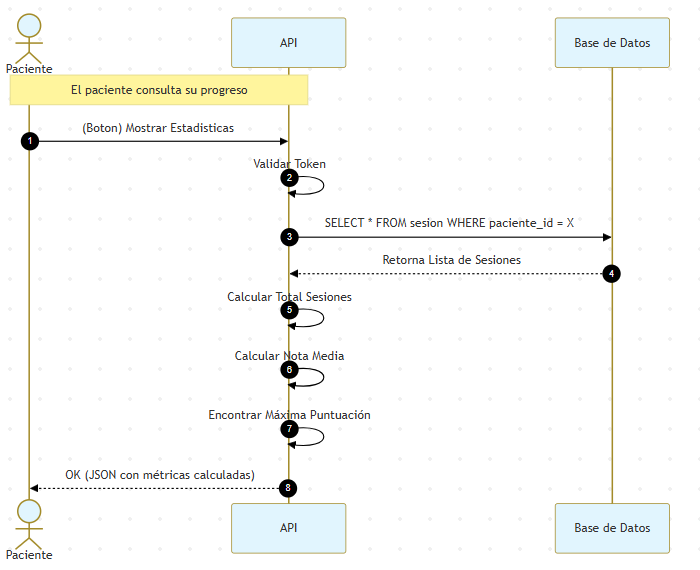
\includegraphics[width=1\textwidth]{img/Diagramas_Secuenciales/DS-consultarprogreso.png}
        \caption{Diagrama de Secuencia: Consulta de Progreso}
        \label{fig:ds_consultar_progreso}
    \end{figure}
\end{enumerate}
\section{Diseño arquitectónico}
El sistema se ha diseñado bajo un esquema de Arquitectura distribuida Cliente-Servidor, utilizando el estilo arquitectónico REST\cite{fielding_rest} (Representational State Transfer) para la comunicación entre los componentes. Esta decisión permite un desacoplamiento total entre la capa de presentación (móvil) y la lógica de negocio y persistencia (backend), facilitando la escalabilidad independiente de ambas partes.

A continuación, se detalla la estructura interna de cada subsistema.

\subsection{Arquitectura global del sistema}
A alto nivel, la solución se compone de tres nodos lógicos diferenciados que interactúan mediante protocolos estándar:

\begin{description}
    \item[Cliente móvil (Android):] actúa como el terminal de usuario (Frontend). Su responsabilidad se limita a la presentación de la interfaz, la captura de sensores (cámara/micrófono) y la solicitud de datos. No procesa reglas de negocio críticas ni almacena datos persistentes a largo plazo (salvo caché).
    
    \item[Servidor de aplicaciones (API REST):] actúa como el núcleo centralizado de la lógica. Expone una interfaz pública mediante HTTP/HTTPS, procesa las peticiones, aplica las reglas de seguridad (autenticación/autorización) y orquesta las transacciones.
    
    \item[Servidor de datos:] nodo pasivo encargado exclusivamente de la persistencia y la integridad referencial de la información relacional.
\end{description}

\subsection{Arquitectura de la aplicación móvil (Patrón MVVM)}
Para el desarrollo del cliente Android, se ha adoptado el patrón de diseño MVVM (Model-View-ViewModel), recomendado por Google en su guía de arquitectura moderna \cite{android_arch_guide}(Modern Android Architecture). Este patrón separa la interfaz de usuario de la lógica de datos, garantizando que la aplicación sea reactiva, testeable y mantenible.

La arquitectura interna de la app se divide en tres capas funcionales:

\begin{enumerate}
    \item \textbf{Capa de interfaz de usuario} \\
    Implementada utilizando Jetpack Compose\cite{jetpack_compose}. A diferencia del sistema de vistas tradicional, esta capa es declarativa.
    \begin{itemize}
        \item Se encarga exclusivamente de ``dibujar'' la pantalla basándose en el estado actual. No contiene lógica de negocio.
        \item La interfaz se reconstruye automáticamente cuando detecta cambios en los datos observables del ViewModel.
    \end{itemize}

    \item \textbf{Capa de lógica de presentación} \\
    Actúa como intermediario entre la vista y los datos.
    \begin{itemize}
        \item Utiliza StateFlow (Kotlin Coroutines) para mantener el estado de la pantalla (ej: ``Cargando'', ``Lista de Pacientes'', ``Error''). La vista se suscribe a este flujo.
        \item Los ViewModels son conscientes del ciclo de vida de Android, sobreviviendo a cambios de configuración (como la rotación de pantalla) para evitar la pérdida de datos temporales.
    \end{itemize}

    \item \textbf{Capa de datos} \\
    Es la capa inferior encargada de la manipulación de datos. Implementa el patrón Repository, que actúa como una ``Fuente Única de Verdad'' (Single Source of Truth).
    \begin{itemize}
        \item El ViewModel solicita datos al Repositorio sin saber de dónde vienen.
        \item El Repositorio decide si obtener los datos de la red o de la persistencia local, encapsulando la complejidad de la sincronización.
    \end{itemize}
\end{enumerate}

\subsection{Arquitectura del servidor}
El backend, desarrollado en FastAPI, sigue una arquitectura estratificada para organizar el código de manera modular.

\begin{description}
    \item[Capa de enrutamiento:] define los endpoints públicos y los verbos HTTP permitidos (GET, POST, PUT, DELETE). Su función es recibir la petición, validar el formato de entrada y delegar la tarea.
    
    \item[Capa de esquemas:] utiliza Pydantic\cite{pydantic_docs} para definir la estructura de los datos que entran y salen de la API. Actúa como un filtro de validación, asegurando que los datos JSON cumplen con los tipos esperados antes de ser procesados.
    
    \item[Capa de modelos:] representa las tablas de la base de datos como objetos Python. Utiliza el ORM (Object-Relational Mapping) para traducir las operaciones lógicas en sentencias SQL, abstrayendo al resto del sistema de la complejidad del lenguaje de consultas.
\end{description}

\section{Diseño de interfaz y experiencia de usuario}
El diseño de la interfaz gráfica de la aplicación no se ha abordado como un mero componente estético, sino como un requisito funcional crítico para el éxito del proyecto. Dado que el sistema está dirigido a pacientes con la enfermedad de Parkinson, el diseño debe compensar las posibles limitaciones motoras (temblores, rigidez, bradicinesia) y cognitivas de los usuarios.

Por ello, la construcción de las vistas se ha regido por los principios de la interacción Persona-Ordenador, priorizando la accesibilidad, la claridad y la minimización de la carga cognitiva sobre la densidad de información. Para la implementación técnica, se ha utilizado el sistema de diseño Material Design 3 de Google, aprovechando las capacidades declarativas del framework Jetpack Compose.

\subsection{Criterios de estilo y adaptación por rol}

La estrategia de diseño visual se ha planteado de forma diferenciada según el perfil del usuario, adaptando la interfaz a las capacidades y necesidades operativas de cada actor:

\begin{description}
    \item[Interfaz del paciente:] dado que este perfil puede presentar limitaciones motoras o visuales, en este módulo se aplican criterios de diseño adaptado. Se utiliza una paleta de alto contraste y se ha sobredimensionado significativamente el tamaño de textos y botones. El objetivo es reducir la precisión necesaria para interactuar con la pantalla y garantizar la legibilidad sin esfuerzo, sacrificando la cantidad de elementos en pantalla en favor de la claridad.
    
    \item[Interfaz de terapeuta y administrador:] para los perfiles profesionales, el diseño se rige por estándares convencionales de productividad. En estas vistas se mantienen los tamaños de fuente y controles estándar de Android para maximizar la densidad de información. Esto permite que el personal sanitario pueda visualizar listados extensos, calendarios y tablas de datos de manera eficiente, evitando el desplazamiento excesivo que provocaría una interfaz sobredimensionada.
\end{description}

\subsection{Arquitectura de la información y navegación}
La estructura de navegación se ha diseñado de forma asimétrica, adaptándose a las necesidades de cada rol:
\begin{itemize}
    \item \textbf{Perfil paciente:} se ha simplificado al extremo la jerarquía. El paciente navega a través de un ``túnel'', eliminando menús complejos, pestañas ocultas o gestos avanzados que requieran motricidad fina.
    \item \textbf{Perfil terapeuta:} mantiene una estructura de árbol estándar de Android, permitiendo la gestión eficiente de múltiples pacientes y recursos.
\end{itemize}

\subsection{Evolución del diseño}
Es fundamental señalar que los diseños presentados en este apartado constituyen la propuesta conceptual inicial. Como es natural en un ciclo de desarrollo ágil, la interfaz final ha divergido en ciertos aspectos respecto a estos planteamientos originales. Durante la fase de implementación técnica, surgieron desafíos y nuevas oportunidades de optimización que obligaron a replantear ciertos flujos para mejorar la eficiencia y la estabilidad del sistema.

Asimismo, la estrategia de desarrollo priorizó en una primera instancia la completitud funcional. El objetivo de estos primeros bocetos y de la versión inicial fue validar la arquitectura lógica y asegurar que todas las funcionalidades críticas —gestión de usuarios, reproducción multimedia y grabación de sesiones— operasen correctamente. Una vez garantizada la robustez operativa, se procedió a fases posteriores de mejora.

Bajo esta premisa de diseño iterativo e incremental, se elaboraron los siguientes bocetos para validar la distribución de elementos. Posteriormente, estos diseños se trasladaron y adaptaron a código mediante Jetpack Compose, dando lugar a la interfaz final.

A continuación, se detalla la estructura planteada para cada perfil de usuario.

\subsubsection{Flujo del administrador}
El diseño para el perfil de administrador se centra en la eficiencia de la gestión de identidades y la supervisión del sistema.(fig.~\ref{fig:boceto_admin_main})

\begin{figure}[hbt]
    \centering
    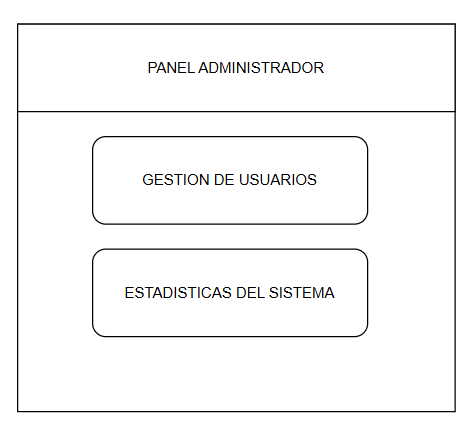
\includegraphics[width=0.8\textwidth]{img/Bocetos/administrador.png}
    \caption{Boceto: panel principal del administrador}
    \label{fig:boceto_admin_main}
\end{figure}

\textbf{Panel principal:} tras la autenticación exitosa, el sistema presenta un panel de control simplificado(fig.~\ref{fig:boceto_admin_main}). Este menú actúa como distribuidor central, segregando claramente las operaciones en dos grandes bloques: ``Gestión de Usuarios'' (operativa diaria) y ``Estadísticas del Sistema'' (monitorización técnica).

\begin{figure}[hbt]
    \centering
    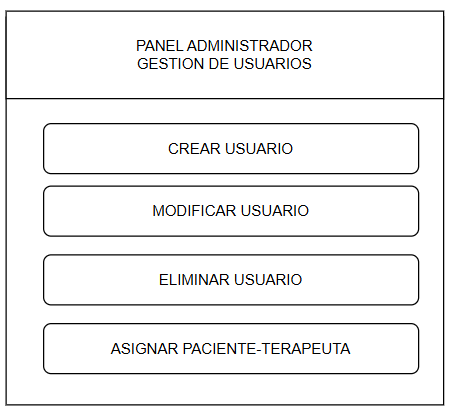
\includegraphics[width=0.8\textwidth]{img/Bocetos/administrador-gestionusuarios.png}
    \caption{Boceto: gestión de usuarios}
    \label{fig:boceto_admin_gestion}
\end{figure}

\textbf{Gestión de usuarios:} al acceder a este módulo, la interfaz despliega las operaciones CRUD (Crear, Leer, Actualizar, Borrar) completas(fig.~\ref{fig:boceto_admin_gestion}). Se diseñaron botones de acceso directo para:

\begin{itemize}
    \item \textbf{Crear, modificar y eliminar de usuarios:} creación de nuevos perfiles o modificación de credenciales existentes.
    \item 
    \item \textbf{Vinculación clínica (Paciente-Terapeuta):} se diseñó una interfaz específica para establecer la relación lógica entre el profesional y el usuario final. Este formulario requiere la selección de un paciente libre y la designación de un terapeuta responsable, garantizando así la integridad referencial y la privacidad de los datos médicos.(fig.~\ref{fig:boceto_admin_asignar})
\end{itemize}

\begin{figure}[hbt]
    \centering
    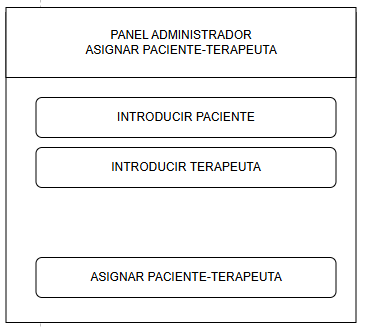
\includegraphics[width=0.8\textwidth]{img/Bocetos/administrador-asignar.png}
    \caption{Boceto: asignación de terapeuta}
    \label{fig:boceto_admin_asignar}
\end{figure}


\subsubsection{Flujo del terapeuta}

\begin{figure}[hbt]
    \centering
    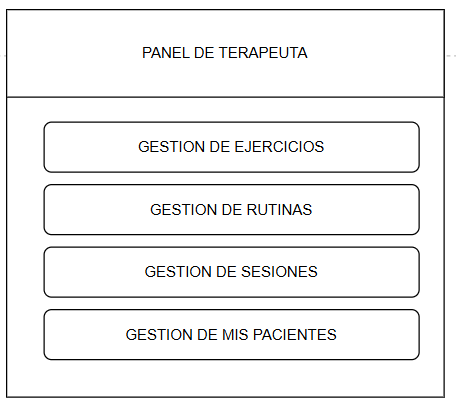
\includegraphics[width=0.8\textwidth]{img/Bocetos/terapeuta.png}
    \caption{Boceto: home del terapeuta}
    \label{fig:boceto_terapeuta_main}
\end{figure}

La interfaz del terapeuta es la más compleja en términos funcionales, ya que debe permitir la gestión integral del tratamiento(fig.~\ref{fig:boceto_terapeuta_main_main}). El diseño modular organiza estas capacidades en cuatro áreas de responsabilidad:

\begin{enumerate}
    \item \textbf{Gestión de ejercicios:} permite administrar la biblioteca multimedia(fig.~\ref{fig:boceto_terapeuta_ejercicios}). El formulario de creación diseñado solicita metadatos críticos: nombre del ejercicio, instrucciones textuales detalladas, duración estimada y, fundamentalmente, el enlace al recurso de vídeo demostrativo.
    
    \begin{figure}[hbt]
        \centering
        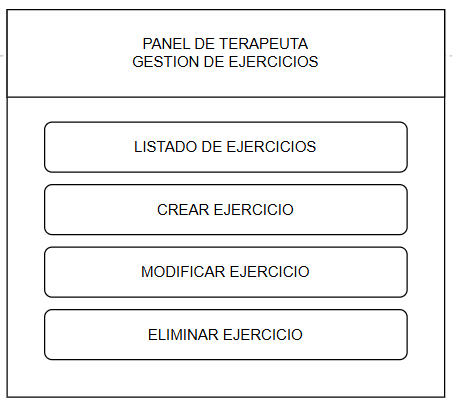
\includegraphics[width=0.45\textwidth]{img/Bocetos/terapeuta-ejercicios.png}
        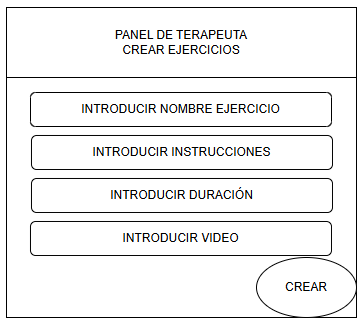
\includegraphics[width=0.45\textwidth]{img/Bocetos/terapeuta-crearejercicio.png}
        \caption{Bocetos: listado y creación de ejercicios}
        \label{fig:boceto_terapeuta_ejercicios}
    \end{figure}

    \item \textbf{Gestión de rutinas:} este módulo permite la agregación lógica(fig.~\ref{fig:boceto_terapeuta_rutinas}). El terapeuta puede consultar el listado de rutinas existentes o componer nuevas plantillas. El diseño contempla la introducción de un nombre, una descripción clínica y la selección secuencial de los ejercicios que compondrán la terapia.

    \begin{figure}[hbt]
        \centering
        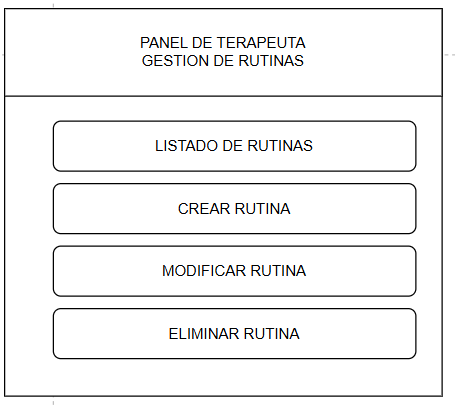
\includegraphics[width=0.45\textwidth]{img/Bocetos/terapeuta-rutinas.png}
        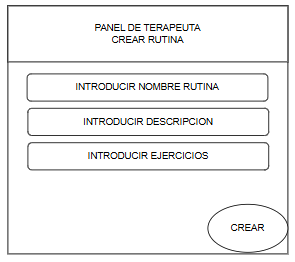
\includegraphics[width=0.45\textwidth]{img/Bocetos/terapeuta-crearrutina.png}
        \caption{Bocetos: gestión de rutinas}
        \label{fig:boceto_terapeuta_rutinas}
    \end{figure}

    \item \textbf{Gestión de sesiones:} es el punto de unión entre el paciente y el tratamiento(fig.~\ref{fig:boceto_terapeuta_sesiones}). La interfaz permite programar una intervención seleccionando tres parámetros clave: el paciente objetivo, la fecha de ejecución y la rutina a aplicar.

    \begin{figure}[hbt]
        \centering
        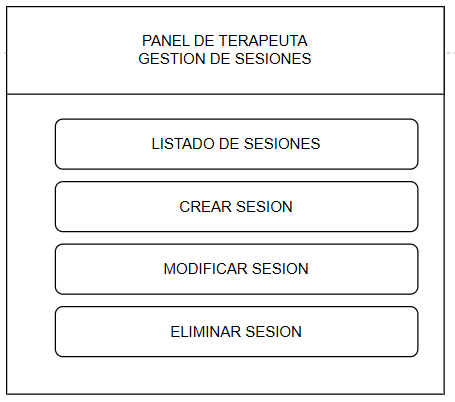
\includegraphics[width=0.45\textwidth]{img/Bocetos/terapeuta-sesiones.png}
        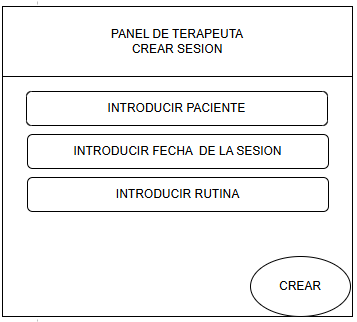
\includegraphics[width=0.45\textwidth]{img/Bocetos/terapeuta-crearsesion.png}
        \caption{Bocetos: programación de sesiones}
        \label{fig:boceto_terapeuta_sesiones}
    \end{figure}

    \item \textbf{Gestión de pacientes:} acceso directo los usuarios asignados.
\end{enumerate}


\subsubsection{Flujo del paciente}
Para el usuario final, el diseño restringe deliberadamente la navegación para minimizar la carga cognitiva y evitar errores operativos.(fig.~\ref{fig:boceto_paciente_inicio})

\textbf{Pantalla de inicio:} la interfaz se reduce a dos únicas acciones primarias representadas por botones de gran tamaño:
\begin{itemize}
    \item \textbf{Entrar a la sesión:} acceso directo a la rutina programada para el día actual. Si no existe programación para la fecha, el sistema gestiona la excepción informando al usuario.
    \item \textbf{Historial:} acceso de solo lectura a las valoraciones pasadas.
\end{itemize}

\begin{figure}[hbt]
    \centering
    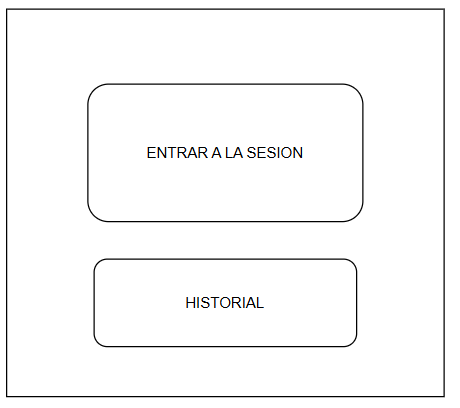
\includegraphics[width=0.8\textwidth]{img/Bocetos/iniciopaciente.png}
    \caption{Boceto: inicio del Paciente}
    \label{fig:boceto_paciente_inicio}
\end{figure}

\textbf{Interfaz de ejecución:} una vez dentro de la sesión, la información se presenta de forma jerarquizada para no abrumar al paciente(fig.~\ref{fig:boceto_paciente_ejecucion}). El flujo sigue una secuencia lógica estricta:
\begin{enumerate}
    \item \textbf{Visualizar ejemplo:} reproducción del vídeo guía.
    \item \textbf{Instrucciones:} lectura de las pautas textuales.
    \item \textbf{Empezar a grabar:} activación de la cámara para registrar la evidencia. Este diseño lineal asegura que el paciente comprenda la tarea antes de intentar realizarla, reduciendo la ansiedad tecnológica.
\end{enumerate}

\begin{figure}[hbt]
    \centering
    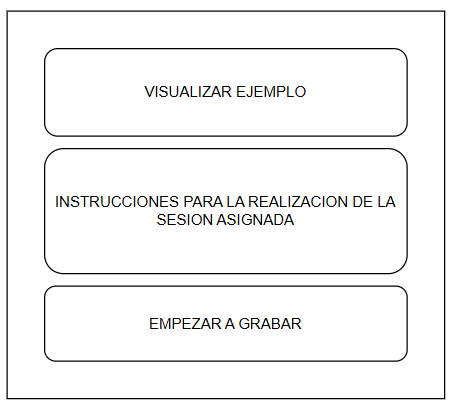
\includegraphics[width=0.8\textwidth]{img/Bocetos/paciente.png}
    \caption{Boceto: interfaz de ejecución del paciente}
    \label{fig:boceto_paciente_ejecucion}
\end{figure}\textbf{}